\subsection{Adaptive tensor learning with tensor networks}


В работе идет речь про тензорные разложения (\textit{ТТ, TR и Tucker}) и  метод \textit{Greedy-TN} поиска оптимального разложения тензора с помощью TensorNetwork для восстановления изображения.
\subsubsection{TensorNetwork} 

\begin{figure}[h!tp]
\centering
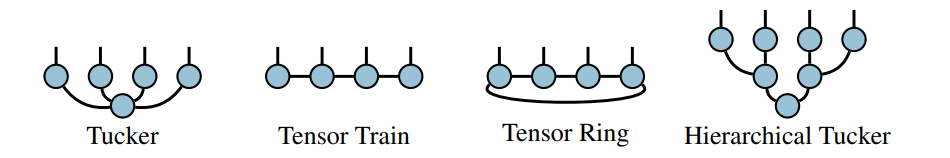
\includegraphics[scale=0.5]{Adaptive tensor learning with tensor networks/DecompTN.PNG}
\caption{Тензорная сеть для тензорных разложений}
\label{fig:TensorNetExamples}
\end{figure}


Построенная тензорная сеть является решением задачи минимизации функции потерь $\mathcal{L}$. 
Рассмотрим пример: $\mathcal{T} \in \mathbb{R}^{d_1 \times d_2 \times d_3 \times d_4}$ - мы хотим его разложить в TT, тогда мы ищем:


\begin{equation}\label{min_tn}
\min\limits_{
\begin{split}
\mathcal{G}^{(1)}\in \mathbb{R}^{d_1 \times r_1 \times 1 \times 1} ; \mathcal{G}^{(2)} \in \mathbb{R}^{r_1 \times d_1 \times r_2 \times 1}; \\  \mathcal{G}^{(3)} \in \mathbb{R}^{1 \times r_2 \times d_3 \times r_3};\mathcal{G}^{(4)} \in \mathbb{R}^{1 \times 1 \times r_3 \times d_4}\end{split}}  \mathcal{L}(TN(\mathcal{G}^{(1)},\mathcal{G}^{(2)},\mathcal{G}^{(3)},\mathcal{G}^{(4)}))
\end{equation}
Но в общем случае тензорная сеть может иметь больше связей и выглядеть, например, вот так:


\begin{figure}[h!tp]
\centering
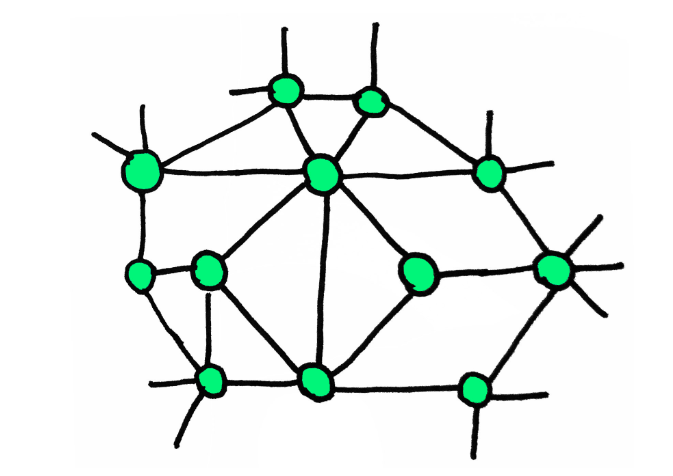
\includegraphics[scale=0.5]{Adaptive tensor learning with tensor networks/TN.PNG}
\caption{Вид тензорной сети}
\label{fig:TensorNetExample}
\end{figure}


\subsubsection{Greedy Algorithm}
Из $\mathcal{T} \in \mathbb{R}^{d_1 \times d_2 \cdots \times d_p}$ строим его приближение core-тензорами $\mathcal{G}^{(i)} \in \mathbb{R}^{R_{1,i} \times \cdots \times R_{i-1,i} \times  d_i \times R_{i,i+1} \times \cdots R_{i,p} }$. 

Операции алгоритма описаны на \ref{fig:GreedyAlg}
\begin{figure}[h!tp]
\centering
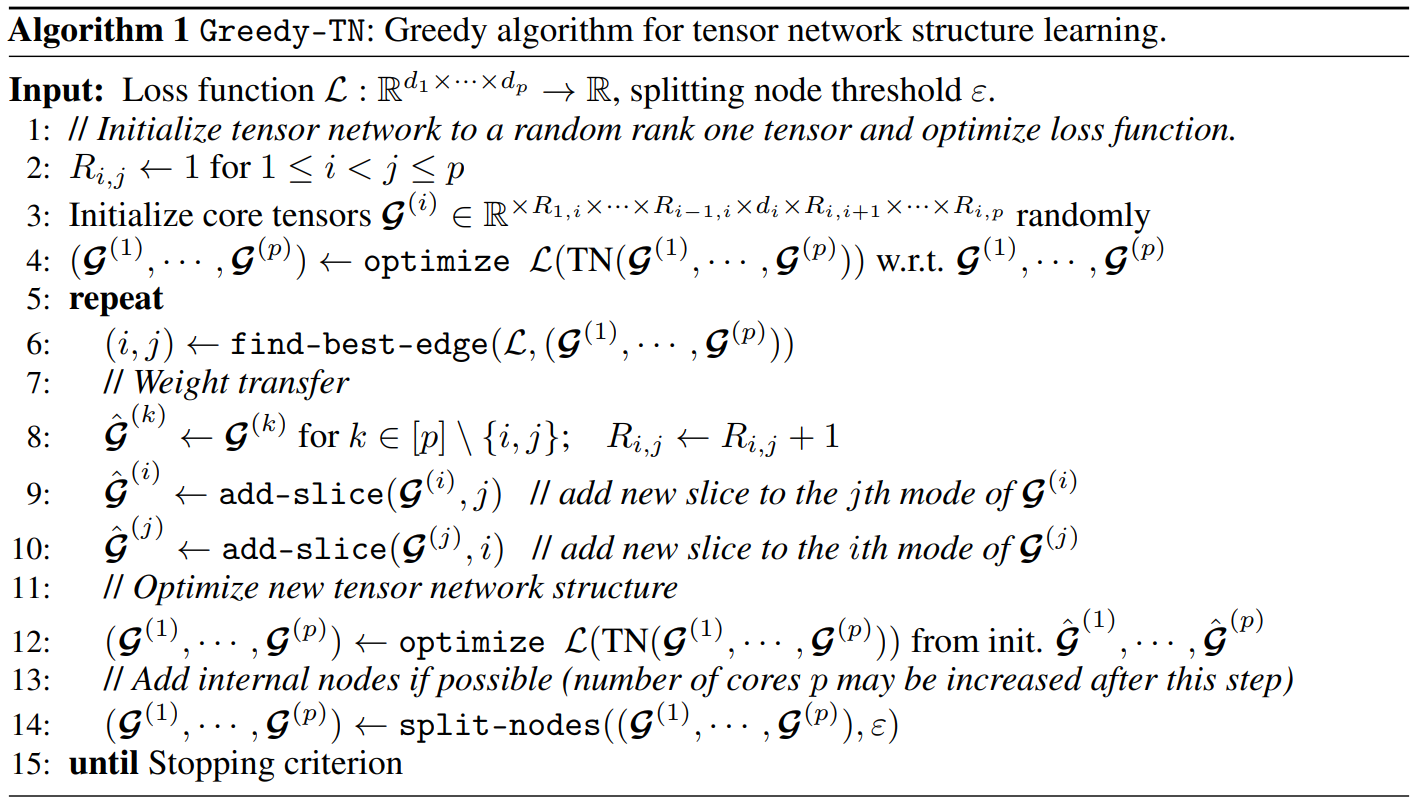
\includegraphics[scale=0.5]{Adaptive tensor learning with tensor networks/alg.PNG}
\caption{Greedy Algorithm}
\label{fig:GreedyAlg}
\end{figure}